\documentclass[11pt]{amsbook}

\usepackage{../HBSuerDemir}	% ------------------------

\begin{document}

% ++++++++++++++++++++++++++++++++++++++
\hPage{b1p2/252}
% ++++++++++++++++++++++++++++++++++++++

in \(R^{n}\), whose coordinates satisfy the equation. Therefore

\[a_{1}s_{1}+a_{2}s_{2}+\dots+a_{n}s_{n}=b\]
\\
If a point is a solution of every equation of the system (2) it is a solution point of the system.
\\
As we shall see, some systems have no solution, some have a unique solution and some others have infinitely many solutions. The system having no solution is said to be \textit{inconsistent}, otherwise \textit{consistent}.
\\
Every HLS has the zero solution point, called the \textit{trivial} solution.
\\
\subsection{Solution by Determinants\(^{(*)}\)}
\label{subsec:SolutionbyDeterminants}
\footnote{(*) Solution matrices will be given in Book II.}
\\

\subsubsection{Square NHLS}:
\label{subsubsec:SquareNHLS}
\\

Let  \[a_{11}x_{1}+\dots+a_{ij}x_{j}+\dots+a_{1n}x_{n}=b_{1}\]
\[\quad\quad\quad\quad\quad\quad\quad\quad
\vdots\quad\quad\quad\quad\quad\quad
\vdots\quad\quad\quad\quad\quad\
\vdots\quad\quad\quad\vdots
\quad(m*n)
\quad\quad\quad(1)
\]
\[a_{n1}x_{1}+\dots+a_{nj}x_{j}+\dots+a_{nn}x_{n}=b_{1}\]

be a square NHLS. The determinant of the coefficients is

\[
D=D_{coeff}= \begin{vmatrix} 
    a_{11} &        & \dots  & a_{1j} &  \dots & a_{1n} \\
    \vdots &        &        & \vdots &        & \vdots \\
    a_{n1} &        & \dots  & a_{nj} &  \dots & a_{nn} \\
    \end{vmatrix}
\]

\begin{thm}[CRAMES's Rule]
	The square system (1) has the unique solution point.

	\[
		\left(
			x_1 = \frac{D_1}{D} , \dots ,
			x_j = \frac{D_j}{D} , \dots ,
			x_n = \frac{D_n}{D}
		\right)
	\]

	if D \(\neq\) 0, and has no solution or infinitely many solution points
	\\
	if D = 0, where D\(_j\) is the determinant obtained from D replacing its jth column by the column of constants.
\end{thm}

% =======================================================
\end{document}  

%==== templates ====

%==== environments ====

%\begin{figure}[htb]
%	\centering
%	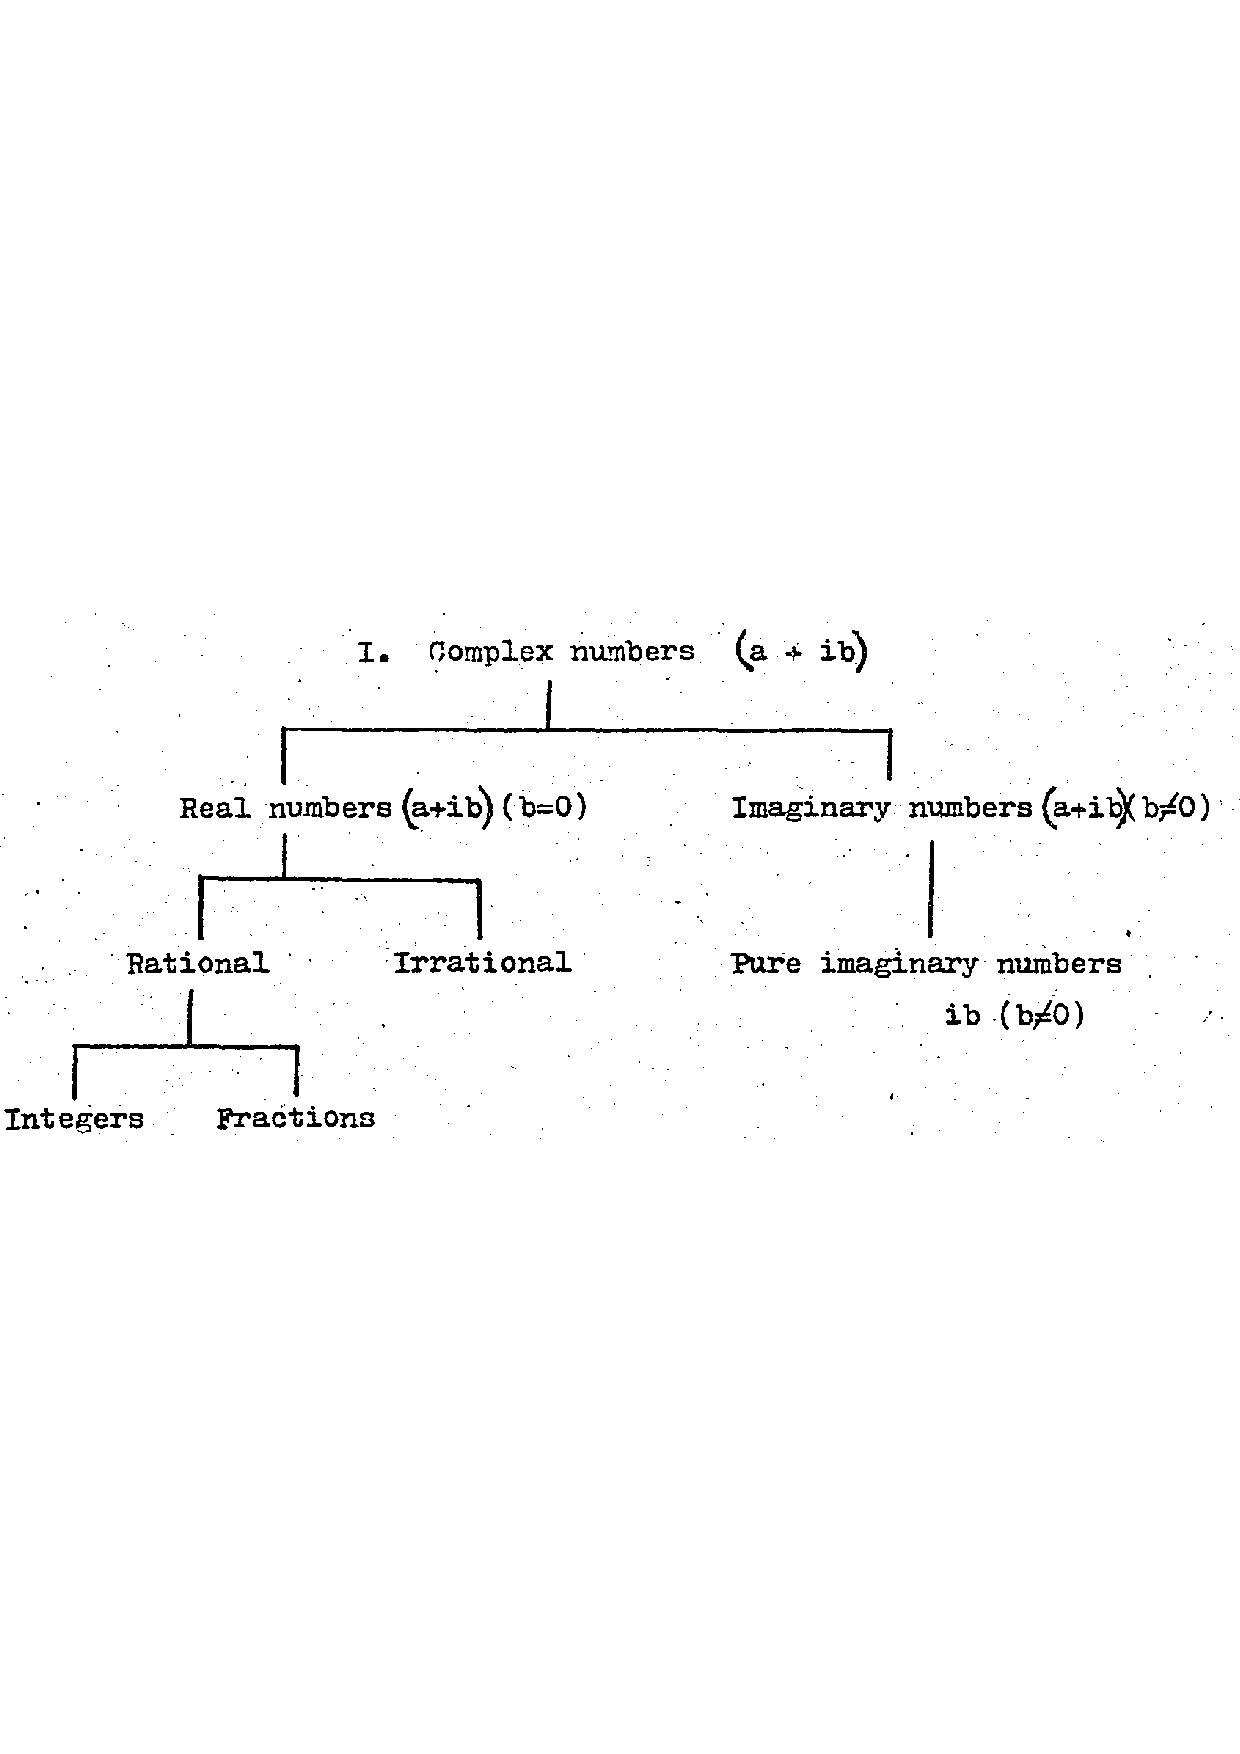
\includegraphics[width=0.9\textwidth]{images/SD-1-1p15A}
%	\caption{Classification of complex numbers}
%	\label{fig:classificationOfComplexNumbersA}
%\end{figure}

%\begin{center}
%\begin{tabular}{cc}
%\end{tabular}
%\end{center}

%\begin{exmp}
%\begin{hSolution}
%\end{hSolution}
%\end{exmp}

%\begin{hEnumerateAlpha}
%\end{hEnumerateAlpha}

%\begin{hEnumerateRoman}
%\end{hEnumerateRoman}

%$
%\begin{bmatrix}
%\end{bmatrix}
%$

%\frac{aaaa}{bbb}
%\frac{a_{n}}{b_{n}}
%\left( aaaa \right)
%\Longrightarrow

%\begin{multicols}{2}
%	bb
%\columnbreak
%	aa
%\end{multicols}
